% Hlavicka pro protokoly z fyzikalniho praktika.
% Verze pro: LaTeX
% Verze hlavicky: 22. 2. 2007
% Autor: Ustav fyziky kondenzovanych latek
% Ke stazeni: www.physics.muni.cz/ufkl/Vyuka/
% Licence: volne k pouziti, nejlepe k vcasnemu odevzdani protokolu z Vaseho mereni.


\documentclass[czech,11pt,a4paper]{article}
\usepackage[T1]{fontenc}
\usepackage{graphicx, animate}
\usepackage{mathtools}
\usepackage{amssymb}
\usepackage{amsthm}
\usepackage{thmtools}
\usepackage{xcolor}
\usepackage{nameref}
\usepackage{babel}
\usepackage{hyperref}
\usepackage{multicol}
\usepackage[export]{adjustbox}
\usepackage{subcaption}
\usepackage{caption}
\usepackage{multirow}
\usepackage{float}
\usepackage{placeins}

\graphicspath{ {./images/} }
\usepackage[backend=biber,style=numeric]{biblatex}       % [1], [2], ...




\addbibresource{ref.bib}


%%% Nemente:
\usepackage[margin=2cm]{geometry}
\newtoks\jmenopraktika \newtoks\jmeno \newtoks\datum
\newtoks\obor \newtoks\skupina \newtoks\rocnik \newtoks\semestr
\newtoks\cisloulohy \newtoks\jmenoulohy

%%% Nemente - konec.


%%%%%%%%%%% Doplnte pozadovane polozky:

\jmenopraktika={Fyzikální praktikum 3}  % nahradte jmenem vaseho predmetu
\jmeno={Teodor Duraković}            % nahradte jmenem mericiho
\datum={8.~dubna 2025}        % nahradte datem mereni ulohy
\obor={F}                     % nahradte zkratkou vami studovaneho oboru
\skupina={Út 14:00}            % nahradte dobou vyuky vasi seminarni skupiny
\rocnik={II}                  % nahradte rocnikem, ve kterem studujete
\semestr={IV}                 % nahradte semestrem, ve kterem studujete

\cisloulohy={9}               % nahradte cislem merene ulohy
\jmenoulohy={Měření činnosti fotonásobiče}           % nahradte vlhkosti vzduchu pri mereni (v %)

%%%%%%%%%%% Konec pozadovanych polozek.


%%%%%%%%%%% Uzitecne balicky:

%%%%%% Zamezeni parchantu:
\widowpenalty 10000 \clubpenalty 10000 \displaywidowpenalty 10000
%%%%%% Parametry pro moznost vsazeni vetsiho poctu obrazku na stranku
\setcounter{topnumber}{3}	  % max. pocet floatu nahore (specifikace t)
\setcounter{bottomnumber}{3}	  % max. pocet floatu dole (specifikace b)
\setcounter{totalnumber}{6}	  % max. pocet floatu na strance celkem
\renewcommand\topfraction{0.9}	  % max podil stranky pro floaty nahore
\renewcommand\bottomfraction{0.9} % max podil stranky pro floaty dole
\renewcommand\textfraction{0.1}	  % min podil stranky, ktery musi obsahovat text
\intextsep=8mm \textfloatsep=8mm  %\intextsep pro ulozeni [h] floatu a \textfloatsep pro [b] or [t]

% Tecky za cisly sekci:
\renewcommand{\thesection}{\arabic{section}.}
\renewcommand{\thesubsection}{\thesection\arabic{subsection}.}
\renewcommand{\thesubsubsection}{\thesubsection\arabic{subsubsection}.}
% Jednopismenna mezera mezi cislem a nazvem kapitoly:
\makeatletter \def\@seccntformat#1{\csname the#1\endcsname\hspace{1ex}} \makeatother


%%%%%%%%%%%%%%%%%%%%%%%%%%%%%%%%%%%%%%%%%%%%%%%%%%%%%%%%%%%%%%%%%%%%%%%%%%%%%%%
%%%%%%%%%%%%%%%%%%%%%%%%%%%%%%%%%%%%%%%%%%%%%%%%%%%%%%%%%%%%%%%%%%%%%%%%%%%%%%%
% Zacatek dokumentu
%%%%%%%%%%%%%%%%%%%%%%%%%%%%%%%%%%%%%%%%%%%%%%%%%%%%%%%%%%%%%%%%%%%%%%%%%%%%%%%
%%%%%%%%%%%%%%%%%%%%%%%%%%%%%%%%%%%%%%%%%%%%%%%%%%%%%%%%%%%%%%%%%%%%%%%%%%%%%%%

\begin{document}
	
	%%%%%%%%%%%%%%%%%%%%%%%%%%%%%%%%%%%%%%%%%%%%%%%%%%%%%%%%%%%%%%%%%%%%%%%%%%%%%%%
	% Nemente:
	%%%%%%%%%%%%%%%%%%%%%%%%%%%%%%%%%%%%%%%%%%%%%%%%%%%%%%%%%%%%%%%%%%%%%%%%%%%%%%%
	\thispagestyle{empty}
	
	{
		\begin{center}
			\sf 
			{\Large Ústav fyziky a technologií plazmatu Přírodovědecké fakulty Masarykovy univerzity} \\
			\bigskip
			{\huge \bfseries FYZIKÁLNÍ PRAKTIKUM} \\
			\bigskip
			{\Large \the\jmenopraktika}
		\end{center}
		
		\bigskip
		
		\sf
		\noindent
		\setlength{\arrayrulewidth}{1pt}
		\begin{tabular*}{\textwidth}{@{\extracolsep{\fill}} l l}
			\large {\bfseries Zpracoval:}  \the\jmeno & \large  {\bfseries Naměřeno:} \the\datum\\[2mm]
			\large  {\bfseries Obor:} \the\obor  \hspace{40mm}  {\bfseries Skupina:} \the\skupina %
			%{\bfseries Ročník:} \the\rocnik \hspace{5mm} {\bfseries Semestr:} \the\semestr  
			&\large {\bfseries Testováno:}\\
			\\
			\hline
		\end{tabular*}
	}
	
	\bigskip
	
	{
		\sf
		\noindent \begin{tabular}{p{3cm} p{0.6\textwidth}}
			\Large  Úloha č. {\bfseries \the\cisloulohy:} \par
			\smallskip
			&\Large \bfseries \the\jmenoulohy  \\[2mm]
		\end{tabular}
	}
	
	\vskip1cm
	
	%%%%%%%%%%%%%%%%%%%%%%%%%%%%%%%%%%%%%%%%%%%%%%%%%%%%%%%%%%%%%%%%%%%%%%%%%%%%%%%
	% konec Nemente.
	%%%%%%%%%%%%%%%%%%%%%%%%%%%%%%%%%%%%%%%%%%%%%%%%%%%%%%%%%%%%%%%%%%%%%%%%%%%%%%%
	
	%%%%%%%%%%%%%%%%%%%%%%%%%%%%%%%%%%%%%%%%%%%%%%%%%%%%%%%%%%%%%%%%%%%%%%%%%%%%%%%
	%%%%%%%%%%%%%%%%%%%%%%%%%%%%%%%%%%%%%%%%%%%%%%%%%%%%%%%%%%%%%%%%%%%%%%%%%%%%%%%
	% Zacatek textu vlastniho protokolu
	%%%%%%%%%%%%%%%%%%%%%%%%%%%%%%%%%%%%%%%%%%%%%%%%%%%%%%%%%%%%%%%%%%%%%%%%%%%%%%%
	%%%%%%%%%%%%%%%%%%%%%%%%%%%%%%%%%%%%%%%%%%%%%%%%%%%%%%%%%%%%%%%%%%%%%%%%%%%%%%%
	
	\begin{multicols}{2}
		\section{Zadání}
		1. Stanovte závislost koeficientu sekundární emise na energii elektronů dopadajícíh na dynodu. Vyneste do grafu i závislost $\ln (\sigma/V) = f(V)$. Zjistěte, jestli koeficient sekundární emise $\sigma$ závisí na intenzitě osvětlení fotokatody.\\
		2. Stanovte a vyneste do grafu závislost integrální citlivosti fotonásobiče a zesílení fotonásobiče na napětí na násobiči $S = f(U_\text{n})\, \text{a} \,M = f(U_\text{n})$.\\
		3. Stanovte integrální citlivost fotokatody $k = f(U_\text{n})$.\\
		4. Prověřte vliv temného proudu na přesnost měření.
		
		
		
		\section{Teorie}
		
		Fotonásobič je vakuová elektrooptická součástka sloužící k detekci velmi slabých světelných signálů. Funguje na principu fotoemise a následného zesílení proudu pomocí sekundární emise elektronů na soustavě dynod. Jeho výstupní signál je úměrný dopadajícímu světelnému toku a použitým napětím, což jej činí mimořádně citlivým detektorem světla pro laboratorní i průmyslové aplikace.
		
		Fotoemise
		Při dopadu světla na fotokatodu dochází k uvolnění elektronů díky vnějšímu fotoefektu. Energie fotonů je přeměněna na kinetickou energii elektronu a překonání výstupní práce materiálu katody. Podle Einsteinova vztahu platí:
		
		\begin{equation} h\nu = w + \frac{1}{2}mv_0^2 \end{equation}
		
		Pro minimální energii potřebnou k emisi elektronu pak definujeme červený práh fotoefektu:
		
		\begin{equation} h\nu_0 = w \end{equation}
		
		Počet emitovaných elektronů je úměrný intenzitě dopadajícího světla za předpokladu neměnného spektrálního složení, což vystihuje Stoletovův zákon:
		
		\begin{equation} I_{\text{f}} = k \cdot \Phi \end{equation}
		kde $I_f$ je proud z fotokatody, $\Phi$ je světelný tok a $k$ je integrální citlivost fotokatody.
		
	\subsection{Sekundární emise}
		Elektrony emitované z fotokatody jsou urychleny napětím a dopadají na první dynodu, kde vyvolávají sekundární emisi. Tento proces se opakuje na každé další dynodě. Koeficient sekundární emise $\sigma$ je definován jako poměr počtu sekundárních elektronů k primárním:
		
		\begin{equation} \sigma = \frac{I_{\text{sek}}}{I_{\text{prim}}} \end{equation}
		
		Závislost koeficientu sekundární emise na energii elektronů dopadajících na dynodu (tj. na napětí mezi dynodami $V$) je dána empirickým vztahem:
		
		\begin{equation} \sigma = A \cdot E \cdot \exp(-\mu E) \end{equation}
		
		kde $E$ je energie elektronů, $A$ a $\mu$ jsou materiálové konstanty.
		
		Předpokládáme-li rovnoměrné napětí mezi dynodami a stejný materiál všech dynod, lze koeficient sekundární emise $\sigma$ určit z proudů měřených na deváté a jedenácté dynodě:
		
		\begin{equation} \sigma = \sqrt{\frac{I_{11}}{I_9}} \end{equation}
		
		Zesílení a citlivost fotonásobiče
		Výsledný anodový proud $I_\mathrm{a}$	je dán zesílením primárního proudu z fotokatody. Za předpokladu, že všechny dynody mají stejný koeficient sekundární emise, platí:
		
		\begin{equation} I_{\text{a}} = \sigma^n \cdot I_{\text{f}} \end{equation}
		
		kde $n$ je počet dynod (v této úloze $n=13$).		
		Zesílení fotonásobiče definujeme jako:
		
		\begin{equation} M = \frac{I_{\text{a}}}{I_{\text{f}}} = \sigma^n \end{equation}
		
		Integrální citlivost fotonásobiče na dopadající světlo je:
		
		\begin{equation} S = \frac{I_{\text{a}}}{\Phi} = M \cdot k \end{equation}
		
		Přepisem obou vztahů získáme:
		
		\begin{equation} I_{\text{a}} = M \cdot k \cdot \Phi = S \cdot \Phi \end{equation}
		
		Pro přímou analýzu závislosti sekundární emise na napětí lze využít logaritmický přepis vzorce:
		
		\begin{equation} \ln\left(\frac{\sigma}{V}\right) = f(V) \end{equation}
		
		kde $V$ je napětí mezi dvěma sousedními dynodami.
		
		\subsection{Temný proud}
		Fotonásobič vykazuje malý proud i bez dopadajícího světla, tzv. temný proud, způsobený především termoemisí. Tento proud je nutné při zpracování dat odečíst, zejména pokud je jeho velikost srovnatelná s měřenými hodnotami.
		
		\section{Měření}
		Nejprve stanovíme hodnotu temných proudů. Z měření závislostí proudů na napětí fotonásobiče Získáváme data pro dynodové proudy i proud anody. Následně tato data fitujeme polynomem III. stupně pro získání spojité závislosti temného proudu na napětí fotonásobiče. Výsledek lze pozorovat na Obr. 1.
		\begin{figure}[H]
			\centering
			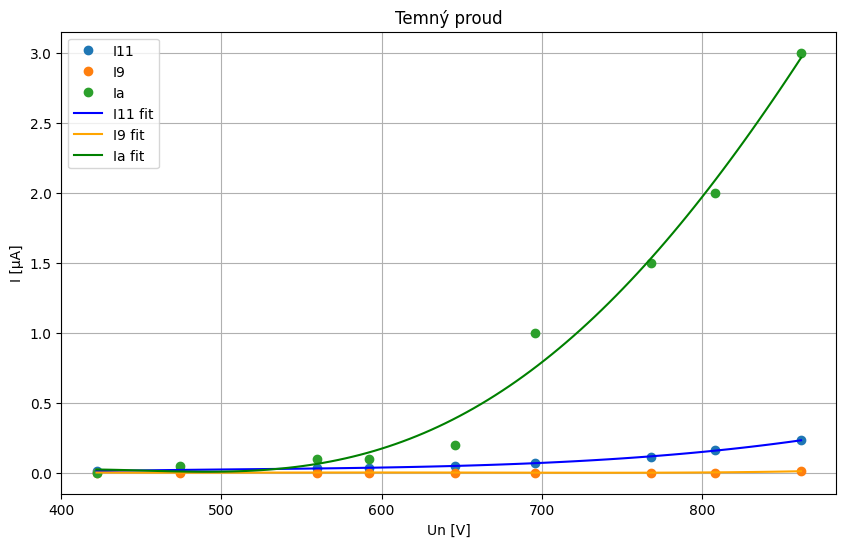
\includegraphics[width=0.9\linewidth]{tp}
			\caption{Závislost měřených temných proudů na napětí}
			
		\end{figure}
		Získané funkcí temného proudu na napětí využíváme pro kompenzaci temného proudu u ostatních měřených dat. Kompenzace dává smysl zejména pro proud $I_9$, tam totiž tvoří až třicet procent měřené hodnoty. U ostatních proudů se jedná o max. jednotky procent
		
		Z měřené závislosti dynodových proudů na napětí mezi dynodami získáváme pomocí formule (6) koeficient sekundární emise. Následně analyzujeme závislost sekundární emise na napětí, získáváme data na obr. 2 a 3. Pozorujeme, že koeficient sekundární emise s napětím roste, což je očekávané.
		
		
		\begin{figure}[H]
			\centering
			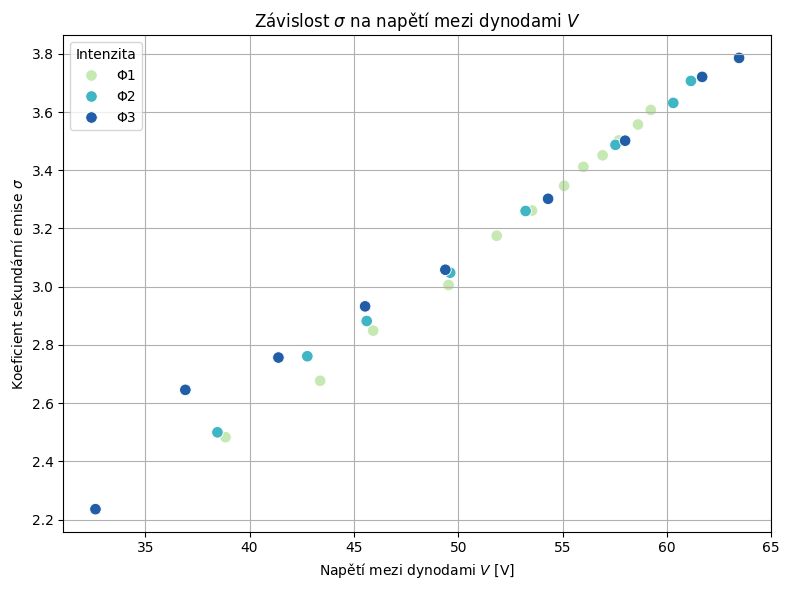
\includegraphics[width=0.9\linewidth]{fig0}
			\caption{Závislost koeficientu sekundární emise na napětí mezi dynodami (energii elektronů), intenzita je úroveň zapuštění optického klínu, index s větším číslem znamená méně dopadajícího světla}
		\end{figure}
		\begin{figure}[H]
			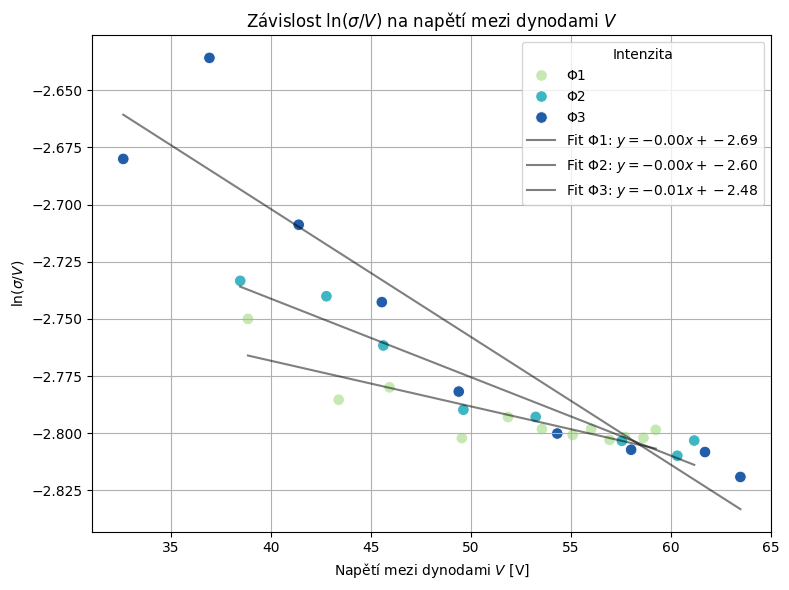
\includegraphics[width=0.9\linewidth]{fig1}
			\caption{závislost logaritmu $\sigma / V$ na napětí mezi dynodami $V$}

		\end{figure}
		Použitím formule (8), resp. (9) získáváme závislosti zesílení, resp. integrální citlivosti fotonásobiče na napětí. Výsledky lze pozorovat na obr. 4 a 5.
		\begin{figure}[H]
			\centering
			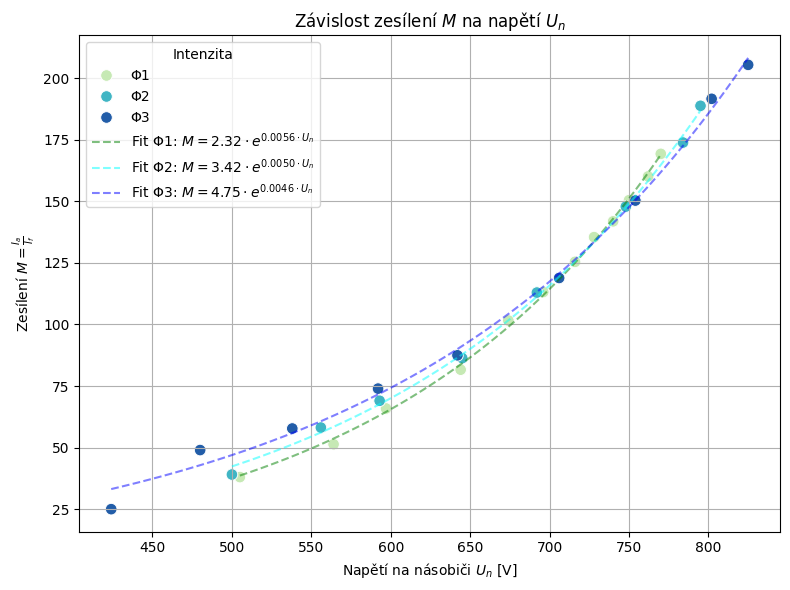
\includegraphics[width=0.9\linewidth]{fig2}
			\caption{Závislost zesílení na napětí}
			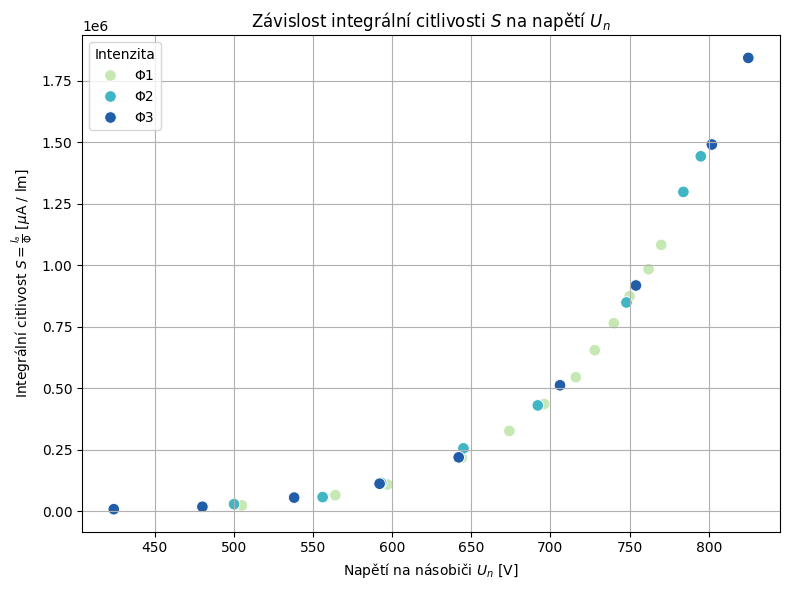
\includegraphics[width=0.9\linewidth]{fig3}
			\caption{Závislost integrální citlivosti na napětí}
			
		\end{figure}
		Jelikož pro integrální citlivost a integrální citlivost fotokatody platí $S = I_a / \Phi$ a $k = I_f / \Phi$, musí platit $k \propto S$.
		\subsection{Integrální citlivost fotokatody}
		Pro měřené závislosti proudů na proměnném světelném toku získáváme konstantu Integrální citlivosti fotokatody pro napětí $600, 750V$, jak lze pozorovat na obr. 6.
		
		\begin{figure}[H]
			\centering
			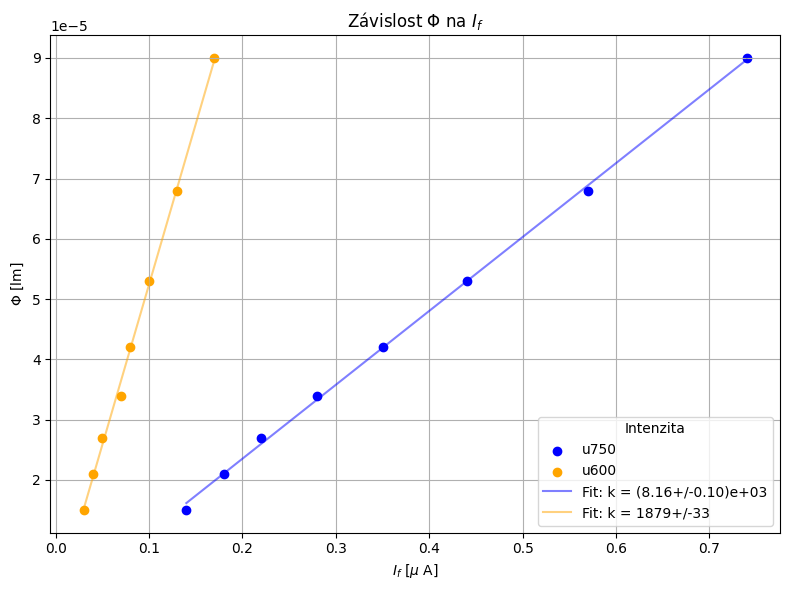
\includegraphics[width=0.9\linewidth]{fig4}
			\caption{Závislost světelného toku na proudu fotokatody}
			
		\end{figure}
		\begin{gather*}
			k_{750} = 8200 \pm 100 \,\mathrm{\mu A \cdot lm ^{-1}}\\
			k_{600} = 1880 \pm 30 \,\mathrm{\mu A \cdot lm ^{-1}}
		\end{gather*}
		
		
		
		
		\section{Závěr}
		Úspěšně se nám podařilo změřit parametry fotonásobiče. Přestože nemáme referenční data, se kterými lze naše výsledky srovnat, dosahují předpokládaných hodnot (zesílení i integrální citlivost s napětím skutečně rostou). 
	\end{multicols}
\printbibliography
			
		
		
		% Nakonec nezapomeňte projet text programem vlna nebo vlnka, např.
		% 	vlna -m -l -n mojeuloha.tex
		% nebo zkontrolovat a opravit jednopísmenné předložky na koncích řádků ručně.

\end{document}
